\documentclass[11pt, a4paper]{article}

\usepackage{amsmath, amssymb, amsthm}
\usepackage{graphicx}
\usepackage{float}
\usepackage{geometry}
\usepackage{hyperref}
\usepackage{booktabs}
\usepackage{cite}

\geometry{margin=2.5cm}

\title{\textbf{Microprice vs Mid-price: \\[4pt]
Does Order Book Imbalance Predict Short-Term Price Moves?}}
\author{Elnoy Greenenko}
\date{April 2026}

\begin{document}
\maketitle

\begin{abstract}
We implement the microprice estimator of Stoikov~\cite{stoikov2018} on live
BTC/USDT order book data from the Binance public API and test whether it
out-predicts the raw mid-price over a 1-second horizon. The microprice adjusts
the mid-price by the order book imbalance at the best bid and ask, shifting
toward the ask when bid-side volume dominates. Over 599 observations collected
at 1-second intervals, the microprice achieves 72\% directional accuracy
against a 50\% coin-flip baseline, confirming that order book imbalance is a
strong short-term predictor of price direction in a liquid market.
\end{abstract}

\section{Introduction}

The mid-price $P^{\text{mid}} = (a + b)/2$ is the standard reference price in
market microstructure, defined as the average of the best ask $a$ and best bid
$b$. It is symmetric by construction: it ignores the relative size of the
resting queues on each side of the book. If there is substantially more resting
buy interest than sell interest, the mid-price understates the true equilibrium
price — the market is more likely to move upward.

The \emph{microprice}, introduced by Stoikov~\cite{stoikov2018}, addresses this
by weighting each price by the opposite side's volume:
\[
P^* = \frac{a V_b + b V_a}{V_a + V_b}.
\]
This is equivalent to
\[
P^* = P^{\text{mid}} + \frac{s}{2} \cdot I,
\]
where $s = a - b$ is the bid-ask spread and
$I = (V_b - V_a)/(V_b + V_a) \in [-1, 1]$ is the \emph{order book imbalance}.
When $I > 0$ (more volume on the bid), $P^* > P^{\text{mid}}$; when $I < 0$,
$P^* < P^{\text{mid}}$.

The central empirical question is: over a 1-second horizon, does the sign of
$(P^* - P^{\text{mid}})$ correctly predict the direction of the next mid-price
move?

\section{Data}

We collect top-of-book snapshots from the Binance public REST API endpoint
\texttt{/api/v3/depth?symbol=BTCUSDT\&limit=5} at 1-second intervals, requiring
no API key. Each snapshot records the best bid price $b$ and volume $V_b$, the
best ask price $a$ and volume $V_a$, and a UTC timestamp. The collection window
covers approximately 10 minutes, yielding 599 usable observations after
applying the forward shift for the prediction target.

Table~\ref{tab:summary} summarises the two key derived quantities. The mean
imbalance of 0.21 is positive, reflecting the upward-trending conditions during
the collection window. The mean spread of \$0.01 on a $\sim$\$78,000 asset
confirms the market is highly liquid — a necessary condition for the imbalance
signal to reflect genuine order flow rather than noise.

\begin{table}[H]
\centering
\begin{tabular}{lcc}
\toprule
 & Imbalance $I$ & Spread $s$ (USDT) \\
\midrule
Mean   & 0.21  & 0.0103 \\
Std    & 0.64  & 0.0054 \\
Min    & $-1.00$ & 0.0100 \\
Max    & $1.00$  & 0.1400 \\
\bottomrule
\end{tabular}
\caption{Summary statistics for order book imbalance and spread,
BTC/USDT, 599 observations.}
\label{tab:summary}
\end{table}

\section{Methodology}

\subsection{Feature engineering}

At each timestamp $t$ we compute:
\[
P^{\text{mid}}_t = \frac{a_t + b_t}{2}, \qquad
P^*_t = \frac{a_t V_{b,t} + b_t V_{a,t}}{V_{a,t} + V_{b,t}}, \qquad
I_t = \frac{V_{b,t} - V_{a,t}}{V_{b,t} + V_{a,t}}.
\]

\subsection{Prediction target and evaluation}

We define the prediction horizon as $h = 1$ row (1 second). The classification
target is $\operatorname{sign}(\Delta P_{t+1})$, where
$\Delta P_{t+1} = P^{\text{mid}}_{t+1} - P^{\text{mid}}_t$.

The microprice signals \emph{up} when $P^*_t > P^{\text{mid}}_t$, equivalently
when $I_t > 0$. We evaluate \textbf{directional accuracy}: the fraction of
non-zero moves for which $\operatorname{sign}(P^*_t - P^{\text{mid}}_t) =
\operatorname{sign}(\Delta P_{t+1})$. Rows with $\Delta P_{t+1} = 0$ are
excluded as they carry no directional information.

\section{Results}

Of the 599 observations, 403 have a non-zero mid-price move at the 1-second
horizon. The microprice achieves 72\% directional accuracy on these observations,
against a 50\% coin-flip baseline (Table~\ref{tab:results}).

\begin{table}[H]
\centering
\begin{tabular}{lc}
\toprule
 & Directional accuracy \\
\midrule
Coin-flip baseline & 50.0\% \\
Microprice signal  & 72.0\% \\
\bottomrule
\end{tabular}
\caption{Directional accuracy over a 1-second horizon, BTC/USDT,
403 non-zero moves from 599 observations.}
\label{tab:results}
\end{table}

Figure~\ref{fig:scatter} shows the relationship between imbalance and future
mid-price change. The bin-mean curve has a clear positive slope — on average, a
more positive imbalance is associated with a larger subsequent upward move —
consistent with the microprice being informative about future price direction.

\begin{figure}[H]
\centering
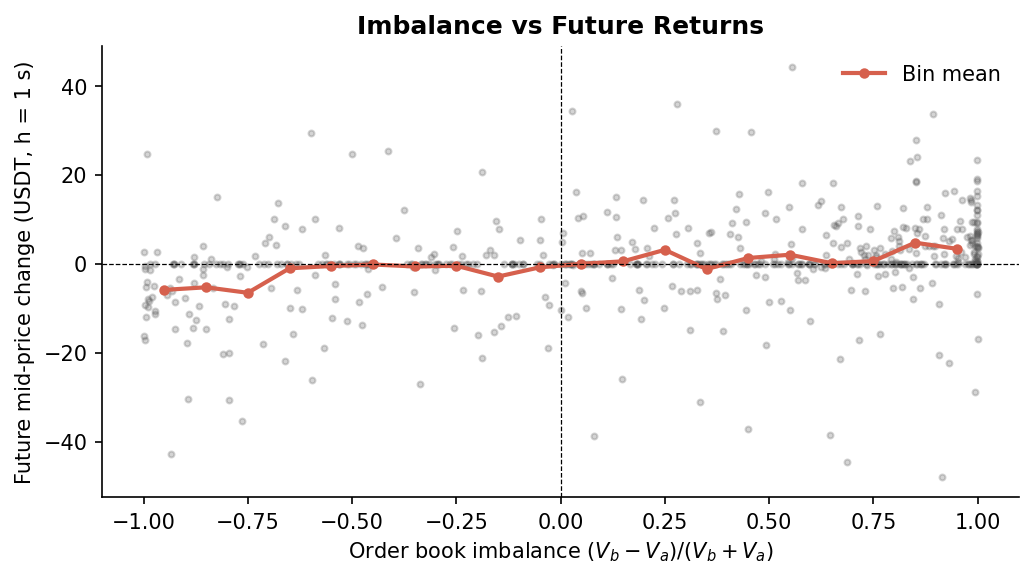
\includegraphics[width=0.75\textwidth]{plots/imbalance_vs_returns.png}
\caption{Scatter of order book imbalance $I_t$ against 1-second forward
mid-price change $\Delta P_{t+1}$. Red line: mean of $\Delta P_{t+1}$ within
each imbalance bin.}
\label{fig:scatter}
\end{figure}

\section{Discussion}

\textbf{Why does the signal work?} When $V_b > V_a$, resting buy interest
exceeds sell interest. Market orders arriving on the ask side consume the
resting bids, pushing the price upward. The microprice encodes this: it shifts
toward the ask in proportion to the imbalance, anticipating the direction of
the move before it happens.

\textbf{Why directional accuracy?} The microprice correction is on the order of
\$1--2 at any given moment. Over a 1-second horizon the price can move
substantially during a volatile period. Directional accuracy isolates the
signal from the noise — it asks only whether the microprice knew which way the
price was going, not how far.

\textbf{Connection to fragmented liquidity.} In a fragmented market, each venue
contributes its own imbalance signal. The aggregated microprice is a
volume-weighted consensus of venue-level signals — the core problem in smart
order routing and liquidity aggregation across fragmented FX pools.

\section{Conclusion}

The microprice provides a simple, parameter-free improvement over the mid-price
as a short-term directional indicator. It requires no model fitting and has a
clean theoretical motivation. The 72\% directional accuracy on live BTC/USDT
data confirms that order book imbalance at the best bid and ask is a strong
predictor of 1-second price direction in a liquid market.

\bibliographystyle{plain}
\begin{thebibliography}{1}
\bibitem{stoikov2018}
Stoikov, S. (2018).
\newblock The micro-price: a high-frequency estimator of future prices.
\newblock \emph{Quantitative Finance}, 18(12), 1959--1966.
\end{thebibliography}

\end{document}